\chapter{Analytic Geometry}


\input section01.01NEW

Much of the mathematics in this chapter will be review for you.  However, the
examples will be oriented toward applications and so 
will take some thought.

\begin{marginfigure}
  \centering
  \begin{tikzpicture}[x=0.2\marginparwidth,y=0.005\marginparwidth]

  \def\xmin{0}
  \def\xmax{4.25}
  \def\ymin{0}
  \def\ymax{95.0}

  % grid
  \draw[style=help lines, ystep=10, xstep=1] (\xmin,\ymin) grid (\xmax,\ymax);

  % axes
  \draw[->] (\xmin,\ymin) -- (\xmax,\ymin) node[right] {$t$};
  \draw[->] (\xmin,\ymin) -- (\xmin,\ymax) node[above] {$h$};

  % xticks and yticks
  \foreach \x in {1,2,...,4}
    \node at (\x, \ymin) [below] {\x};
  \foreach \y in {10,20,...,90}
    \node at (\xmin,\y) [left] {\y};

  \draw[color=black] plot[smooth,mark=*,mark size=1pt] (0,80.0);
  \draw[color=black] plot[smooth,mark=*,mark size=1pt] (1,75.1);
  \draw[color=black] plot[smooth,mark=*,mark size=1pt] (2,60.4);
  \draw[color=black] plot[smooth,mark=*,mark size=1pt] (3,35.9);
  \draw[color=black] plot[smooth,mark=*,mark size=1pt] (4,1.6);

  % generate and plot another a curve y = 0.1 x^2 + 2.5
  % this generates the files figure.parabola.gnuplot and figure.parabola.table 
%  \draw[color=red, domain=\xmin:\xmax] plot[id=parabola]
%  function{0.1*x**2 + 2.5} node [right] {$y=0.1\,x^2 + 2.5$};

\end{tikzpicture}
  \caption{Height versus time.}
  \label{fig:data plot}
\end{marginfigure}

In the $(x,y)$ coordinate system we normally write the $x$-axis
horizontally, with positive numbers to the right of the origin, and
the $y$-axis vertically, with positive numbers above the origin.  That
is, unless stated otherwise, we take ``rightward'' to be the positive
$x$-direction and ``upward'' to be the positive $y$-direction.  In a
purely mathematical situation, we normally choose the same scale for
the $x$- and $y$-axes.  For example, the line joining the origin to
the point $(a,a)$ makes an angle of 45${}^\circ$ with the $x$-axis
(and also with the $y$-axis).

\begin{margintable}
  \centering
  \begin{tabular}{lr}
    \toprule
    $t~\text{(sec)}$ & $s~\text{(meters)}$ \\
    \midrule
    0 &80.0 \\
    1 &75.1 \\
    2 &60.4 \\
    3 & 35.9 \\
    4 & 1.6 \\
    \bottomrule \\
  \end{tabular}
  \caption{A data table.}
  \label{table:data table}
\end{margintable}

In applications, often letters other than $x$ and $y$ are used, and
often different scales are chosen in the horizontal and vertical
directions.  For example, suppose you drop something from a window,
and you want to study how its height above the ground changes from
second to second.  It is natural to let the letter $t$ denote the time
(the number of seconds since the object was released) and to let the
letter $h$ denote the height.  For each $t$ (say, at one-second
intervals) you have a corresponding height $h$.  This information can
be tabulated, and then plotted on the $(t,h)$ coordinate plane, as
shown in Figure~\ref{fig:data plot}.

We use the word ``quadrant''\index{quadrant} for each of the four
regions into which the plane is divided by the axes: the first
quadrant is where points have both coordinates positive, or the
``northeast'' portion of the plot, and the second, third, and fourth
quadrants are counted off counterclockwise, so the second quadrant is
the northwest, the third is the southwest, and the fourth is the
southeast.

\begin{marginfigure}
  
\begin{tikzpicture}[x=0.5\marginparwidth,y=0.5\marginparwidth]
    \draw[->] (0,-1) -- (0,1);
    \draw[->] (-1,0) -- (1,0);
    \node at (0.5,0.5) {\large I};
    \node at (-0.5,0.5) {\large II};
    \node at (-0.5,-0.5) {\large III};
    \node at (0.5,-0.5) {\large IV};
  \end{tikzpicture}
  \caption{The four quadrants.}
  \label{figure:quadrants}
\end{marginfigure}

Suppose we have two points $A$ and $B$ in the $(x,y)$-plane.
We often want to know the change in $x$-coordinate (also called the
``horizontal distance'') in going from $A$ to $B$.  This is often
written $\Delta x$, where the meaning of $\Delta$ (a capital delta in
the Greek alphabet) is ``change in''. (Thus, $\Delta x$ can be read as
``change in $x$'' although it usually is read as ``delta $x$''. The
point is that $\Delta x$ denotes a single number, and should not be
interpreted as ``delta times $x$''.)  
For example, if $A=(2,1)$ and $B=(3,3)$, $\Delta
x=3-2=1$.  Similarly, the ``change in $y$'' is written $\Delta y$.  In
our example, $\Delta y= 3-1=2$, the difference between the
$y$-coordinates of the two points.  It is the vertical distance you
have to move in going from $A$ to $B$.  The general formulas for the
change in $x$ and the change in $y$ between a point $(x_1,y_1)$ and a
point $(x_2,y_2)$ are:
$$
\Delta x=x_2-x_1,\qquad\qquad\Delta y=y_2-y_1.
$$
Note that either or both of these might be negative.

\input section01.01
\input section01.02
\input section01.03
\input section01.04
